\chapter{Implementation} \label{sec:ch_implementation}

This chapter provides the most important implementation details, it is, again, divided into four main sections that correspond the four topics of this thesis.

%%%%%%%%%%%%%%%%%%%%%%%%%%%%%%%%%%%%%%%%%%%%%%%%%%%%%%%%%%%%%%%%%%%%%%%%%%%%%%%%%%%%%
%%%%%%%%%%%%%%%%%%%%%%%%%%%%%%%%%%%%%%%%%%%%%%%%%%%%%%%%%%%%%%%%%%%%%%%%%%%%%%%%%%%%%
\section{Manual Design of Extraction Rules} \label{sec:manual_impl_rules} \graphicspath{{../img/ch50/}}


\subsection{Procedural Extraction Rules} \label{sec:manual_Procedural_Extraction_Rules} 

Our earliest extraction method, which is based on procedural extraction rules, was implemented using Btred\footnote{See details about Btred in Section~\ref{sec:third_tred}.} API for processing linguistic trees. The extraction rules were implemented in Perl as Btred procedures. Application of these extraction rules on a corpus of linguistic trees is realized such that each procedure (or extraction rule) is executed on every available tree by Btred. 

An example of such extraction rule is in Figure~\ref{fig:btred_rule} and corresponding extraction output on Figure~\ref{fig:btred_xml}. Let us briefly describe this extraction rule. The execution is configured such that the procedure of a particular extraction rule (`print\_injured’ on the line 5 in the presented case) is repeatedly called for all nodes of all available trees and the variable `\$this` always contains a reference to the actual tree node. 

The procedure starts with testing if the actual node is a verb (line 6) and if it is one of the intended verbs (lines 7, 8 and 3). If these tests succeed, the rule is applied and following information is printed to the output:
\begin{description}
	\item[<action> enclosing element and its type (line 10)]: the actual verb, that triggered this extraction rule, is used as the type of the action.
	\item[<sentence> (lines 13, 14)]: the full sentence and its \emph{id}.
	\item[<negation> (lines 17-21)]: test whether negation is present or not (e.g. ``truck driver \myemph{did not} survive the accident.’’)
	\item[<manner> (lines 24-29)]: looks for a word expressing the manner of injury (e.g. ``driver was \myemph{seriously} injured.’’)
	\item[<participant> (lines 32-51)]: looks for all participants attached to the action.
	\item[<quantity> of participants (lines 39-44)]: looks for a numeral expressing the quantity of participants (e.g. ``\myemph{two} people died.’’)
	\item[<full\_string> representation of given participant (lines 46-48)]: all words attached to the particular participant node (e.g. ``\myemph{fifteen years old woman} died.’’)
\end{description}





%%%%%%%%%%%%%%%%%%%%%%%%%%%%%%%%%%%%%%%%%%%%%%%%%%%%%%%%%%%%%%%%%%%%%%%%%%%%%%%%%%%%%
\begin{figure}
\begin{minted}[linenos,  fontsize=\footnotesize,
               frame=lines,tabsize=2]{perl}
#variable $this contains currently processed node, $root current root node

my @injure_verbs = ("zranit", "usmrtit", "zemřít", "zahynout", "přežít");
# transcript:       "injure"  "kill"     "die"     "perish"    "survive"
sub print_injured {
	if ($this->{gram}{sempos} eq "v") {
		foreach my $v (@injure_verbs) {
			if ($this->{t_lemma} eq $v ) {
				#action type
				print "<action type=\"" . $this->{t_lemma} . "\">";

				#sentece
				print "<sentece>" . PML_T::GetSentenceString($root) . "</sentece>";
				print "<sentece_id>" . $root->{id} . "</sentece_id>";
				
				#negation
				if (test_negation($this)) {
					print "<negation>true</negation>" ;					
				} else {
					print "<negation>false</negation>" ;										
				}
								
				#manner of injury
				my @mans = find_node_by_attr_depth($this, 0, 'functor', '^MANN');
				if (@mans) {
					foreach my $m (@mans) {
						print "<manner>"; print $m->{t_lemma}; print "</manner>"; 
					};
				}
				
				#actors and patients
				my @pats = find_node_by_attr($this, 'functor', '^[PA][AC]T');
				@pats = &filter_list(\&test_person, @pats);
				
				foreach my $p (@pats) {
					print "<participant type=\"" . $p->{t_lemma} . "\">";

					#participants count
					my @cnt = find_node_by_attr($p, 'functor', '^RSTR');
					@cnt = &filter_list(\&test_number_lemma, @cnt);
					my $cnt1 = pop(@cnt);
					print "<quantity>" . 
						&test_number($cnt1->{t_lemma}) . 
						"</quantity>" if ($cnt1);
	
					print "<full_string>";
					print_subtree_as_text($p);
					print "</full_string>";

					print "</participant>";
				}
				
				#action end
				print "</action>\n";											
}}}}
\end{minted} 
																																		\begin{comment}
																																		this >>$<< hacks my syntax highlighter :-)
																																		\end{comment}
\caption{Procedurally written extraction rule in \emph{Btred}.}
\label{fig:btred_rule}
\end{figure}
%%%%%%%%%%%%%%%%%%%%%%%%%%%%%%%%%%%%%%%%%%%%%%%%%%%%%%%%%%%%%%%%%%%%%%%%%%%%%%%%%%%%%




%%%%%%%%%%%%%%%%%%%%%%%%%%%%%%%%%%%%%%%%%%%%%%%%%%%%%%%%%%%%%%%%%%%%%%%%%%%%%%%%%%%%%
\begin{figure}
\begin{minted}[linenos,  fontsize=\footnotesize,
               frame=lines, tabsize=2]{xml}
<injured_result>
	<action type="zranit">
		<sentece>
			Při požáru byla jedna osoba lehce zraněna -- jednalo se
			o majitele domu, který si vykloubil rameno.
		</sentece>
		<sentece_id>T-vysocina63466.txt-001-p1s4</sentece_id>
		<negation>false</negation>
		<manner>lehký</manner>
		<participant type="osoba">
			<quantity>1</quantity>
			<full_string>jedna osoba</full_string>
		</participant>
	</action>
	<action type="zemřít">
		<sentece>
			Ve zdemolovaném trabantu na místě zemřeli dva muži -- 82letý
			senior a další muž, jehož totožnost zjišťují policisté.
		</sentece>
		<sentece_id>T-jihomoravsky49640.txt-001-p1s4</sentece_id>
		<negation>false</negation>
		<participant type="muž">
			<quantity>2</quantity>
			<full_string>dva muži</full_string>
		</participant>
	</action>
		<action type="zranit">
		<sentece>čtyřiatřicetiletý řidič nebyl zraněn.</sentece>
		<sentece_id>T-jihomoravsky49736.txt-001-p4s3</sentece_id>
		<negation>true</negation>
		<participant type="řidič">
			<full_string>čtyřiatřicetiletý řidič</full_string>
		</participant>
	</action>
</injured_result>
\end{minted}
\caption{\emph{XML} structured output of the query written in \emph{Btred}.}
\label{fig:btred_xml}
\end{figure}
%%%%%%%%%%%%%%%%%%%%%%%%%%%%%%%%%%%%%%%%%%%%%%%%%%%%%%%%%%%%%%%%%%%%%%%%%%%%%%%%%%%%%





\subsection{Netgraph Based Extraction Rules} \label{sec:manual_Netgraph_Based_Extraction_Rules}

Our second extraction method, which is based on Netgraph (see Section~\ref{sec:third_netgraph} for details), is implemented in Java. Java was chosen partly because we use the Java implementation of Netgraph client as a library. 



The extraction is implemented as follows: Netgraph implementation is responsible for the evaluation of the Netgraph query part of extraction rules and matching trees are then returned to our implementation, which prepares the extraction output based on the SELECT part of extraction rules.




\begin{figure}
	\centering
		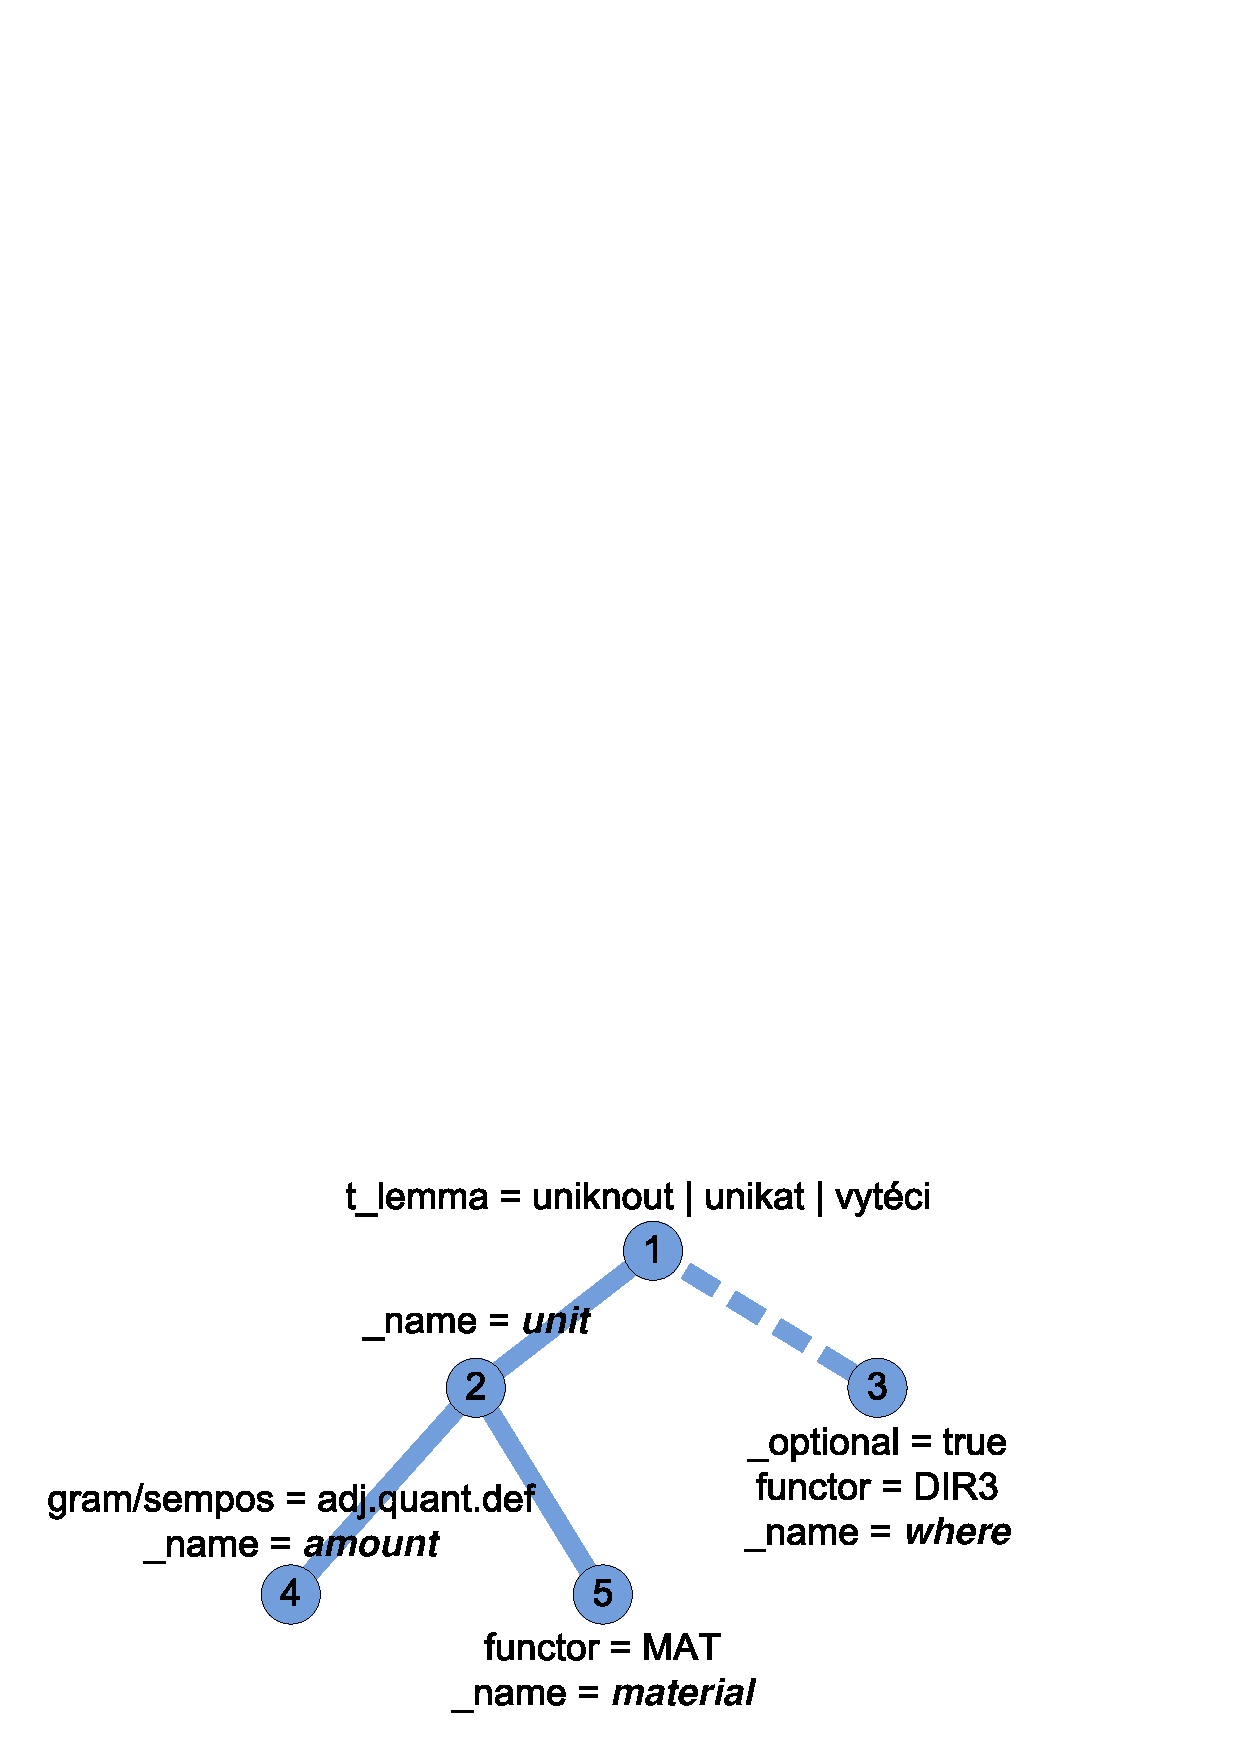
\includegraphics[width=0.5\hsize]{eenv_extract_patern}
\\Transcript:\\
\begin{tabular}{|c|c|}
\hline
uniknout, unikat & vytéci\\
to leak out & to flow out\\
\hline
\end{tabular}		
	\caption{A manually created extraction rule investigating dangerous liquids that spilled out into the environment.}
	\label{fig:manual_eenv_extract_patern}
\end{figure}


\begin{figure}
	\centering
		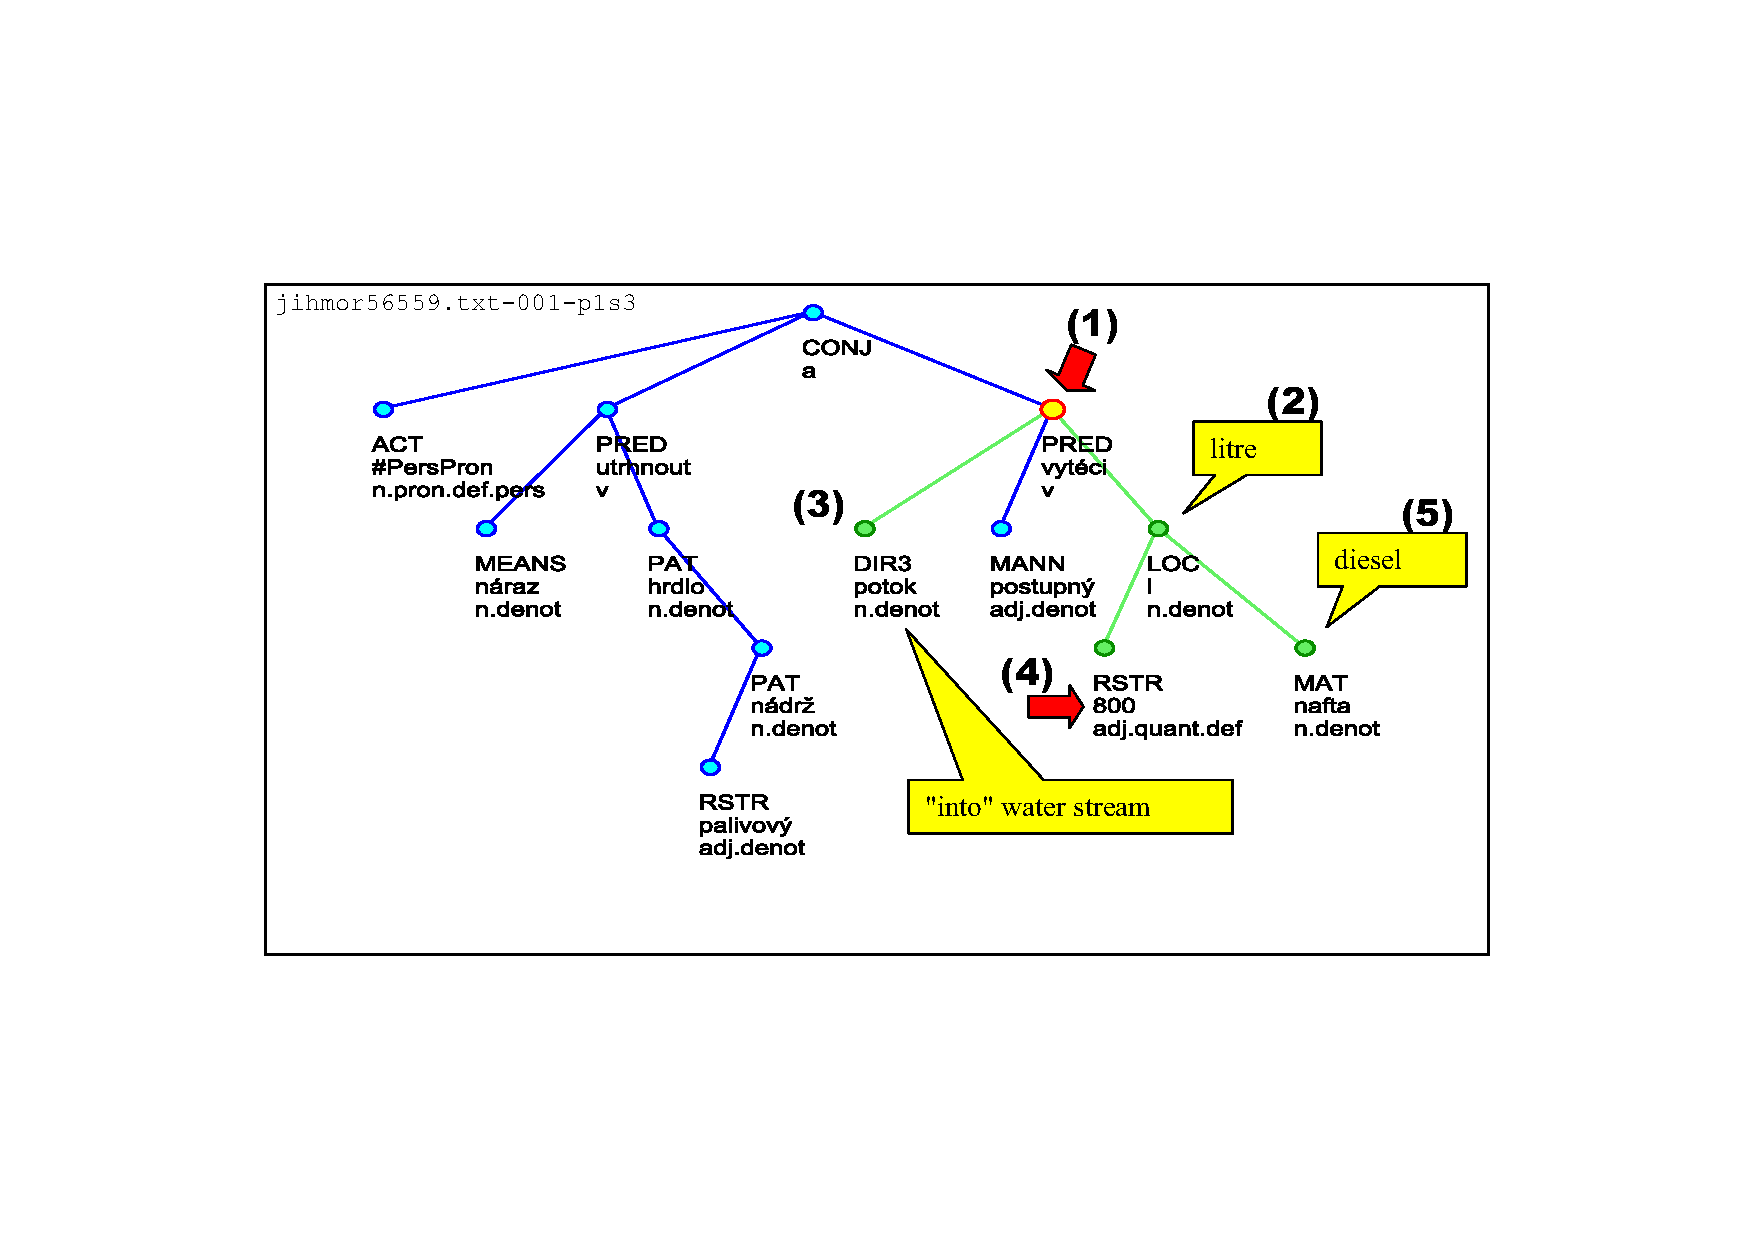
\includegraphics[angle=-90, width=0.6\hsize]{eenv_matching_tree}
		
Original sentence: 
\emph{``Nárazem se utrhl hrdlo palivové nádrže a do potoka postupně vyteklo na 800 litrů nafty.''}\\
English transcript: 
\emph{``Due to the clash the throat of fuel tank tore off and 800 liters of oil (diesel) has run out to a stream.''}
	\caption{A tree matching with the corresponding extraction rule in Figure~\ref{fig:manual_eenv_extract_patern}.}
	\label{fig:manual_eenv_matching_tree}
\end{figure}


%%%%%%%%%%%%%%%%%%%%%%%%%%%%%%%%%%%%%%%%%%%%%%%%%%%%%%%%%%%%%%%%%%%%%%%%%%%%%%%%%%%%%
\begin{figure}
\begin{minted}[linenos,  fontsize=\footnotesize,
               frame=lines, tabsize=2]{xml}
<QueryMatches>
	<Match root_id="T-vysocina63466.txt-001-p1s4" match_string="2:0,7:3,8:4,11:2">
		<Sentence>
			Při požáru byla jedna osoba lehce zraněna - jednalo se
			o majitele domu, který si vykloubil rameno.
		</Sentence>
		<Data>
			<Value variable_name="action_type" attribute_name="t_lemma">zranit</Value>
			<Value variable_name="injury_manner" attribute_name="t_lemma">lehký</Value>
			<Value variable_name="participant" attribute_name="t_lemma">osoba</Value>
			<Value variable_name="quantity" attribute_name="t_lemma">jeden</Value>
		</Data>
	</Match>
	<Match root_id="T-jihomoravsky49640.txt-001-p1s4" match_string="1:0,13:3,14:4">
		<Sentence>
			Ve zdemolovaném trabantu na místě zemřeli dva muži - 82letý senior
			a další muž, jehož totožnost zjišťují policisté.
		</Sentence>
		<Data>
			<Value variable_name="action_type" attribute_name="t_lemma">zemřít</Value>
			<Value variable_name="participant" attribute_name="t_lemma">muž</Value>
			<Value variable_name="quantity" attribute_name="t_lemma">dva</Value>
		</Data>
	</Match>
	<Match root_id="T-jihomoravsky49736.txt-001-p4s3" match_string="1:0,3:3,7:1">
		<Sentence>Čtyřiatřicetiletý řidič nebyl zraněn.</Sentence>
		<Data>
			<Value variable_name="action_type" attribute_name="t_lemma">zranit</Value>
			<Value variable_name="a-negation" 
			       attribute_name="m/tag">VpYS---XR-NA---</Value>
			<Value variable_name="participant" attribute_name="t_lemma">řidič</Value>
		</Data>
	</Match>
</QueryMatches>
\end{minted}
\caption{\emph{XML} structured output of the SQL select like query. A negation can be detected from the presence of \emph{m/tag} on the line 30.}
\label{fig:select_xml}
\end{figure}
%%%%%%%%%%%%%%%%%%%%%%%%%%%%%%%%%%%%%%%%%%%%%%%%%%%%%%%%%%%%%%%%%%%%%%%%%%%%%%%%%%%%%

\begin{figure}
	\centering
		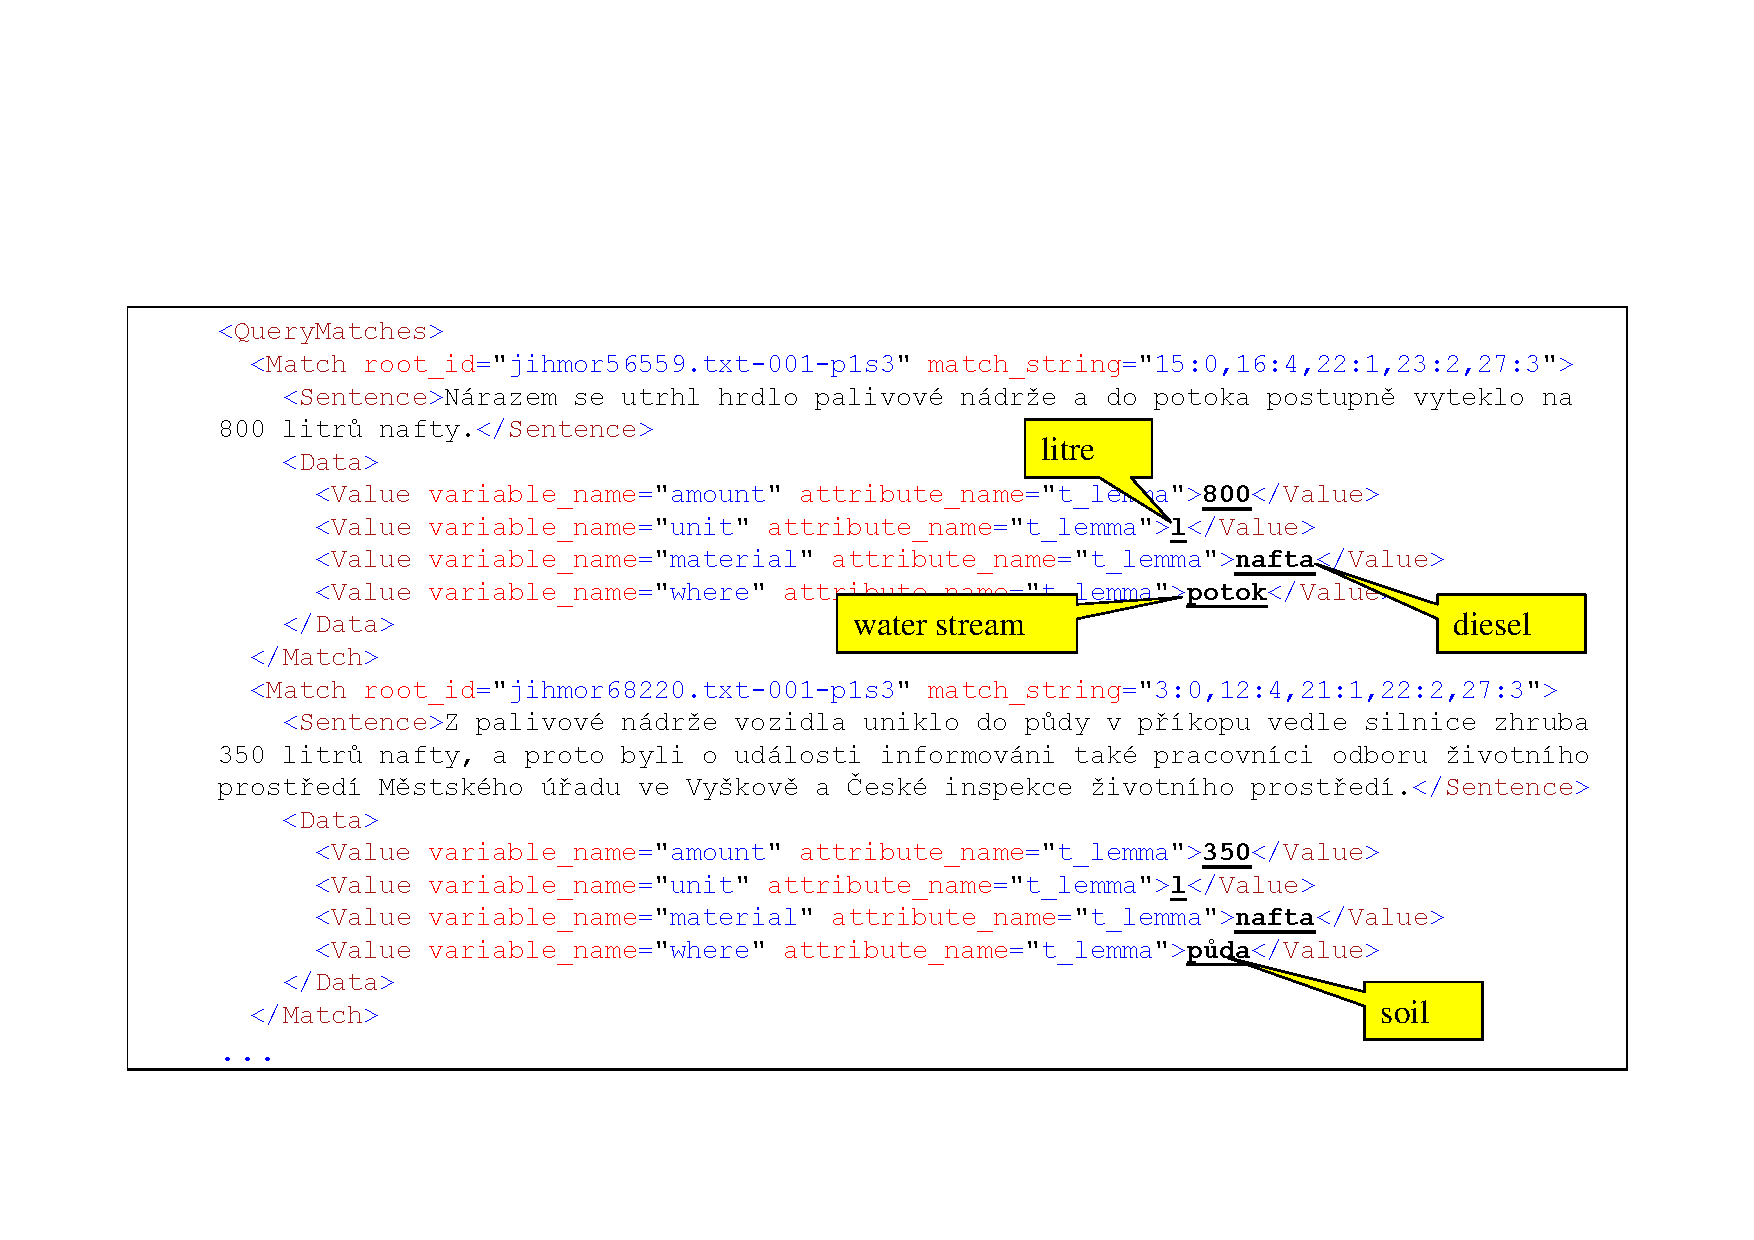
\includegraphics[angle=-90, width=0.7\hsize]{eenv_results}
	\caption{\emph{XML} structured output of the SQL select like query corresponding with the extraction rule in Figure~\ref{fig:manual_eenv_extract_patern} and matching tree in Figure~\ref{fig:manual_eenv_matching_tree}.}
	\label{fig:manual_eenv_results}
\end{figure}























\subsubsection{Illustration Examples}



Evaluation of the extraction rule from Figure~\ref{fig:manual_eenv_extract_patern} is illustrated on Figure~\ref{fig:manual_eenv_matching_tree}. Figure~\ref{fig:manual_eenv_matching_tree} shows a linguistic tree matching with the extraction rule. Matching nodes are decorated and labeled by the numbers of corresponding query nodes.



\subsection{Extraction Output} \label{sec:manual_impl_output}

Small pieces of extraction outputs are shown in Figure~\ref{fig:select_xml} (for the extraction rule in Figure~\ref{fig:manual_extract_patern}) and in Figure~\ref{fig:manual_eenv_results} (for the extraction rule in Figure~\ref{fig:manual_eenv_extract_patern}). 

The former example (Figure~\ref{fig:select_xml}) contains three matches of the extraction rule in three different articles. Each query match is closed in the \verb+<Match>+ element and each contains values of some linguistic attributes closed inside the \verb+<Value>+ elements. Each value comes from some of the nodes of the extraction rule. Name of corresponding query node is saved in the \verb+variable_name+ attribute of the \verb+<Value>+ element.

In the case of the example query, values identified by the variable \verb+action_type+ specify the type of the action. So in the first and third case somebody was injured (\emph{zranit} means to injure in Czech, lines 8 and 28) and in the second case somebody died (\emph{zemřít} means to die in Czech, line 20).

Values identified by \verb+participant+ and \verb+quantity+ contain information about participants of the action. \verb+participant+ serves for specification of the type of the participants and \verb+quantity+ values hold numbers (quantity) of the participants. So in the first action one (\emph{jeden}, line 11) person (\emph{osoba}, line 10) was injured and in the second action two (\emph{dva}, line 22) men (\emph{muž}, line 21) died.

Values identified by \verb+a-negation+ contain the information about a negation of a clause (The presence of negation is indicated by the 11th character of the position-based morphological tag, note that the corresponding node (number 2) of the extraction rule is marked as optional and the restriction on m/tag is put in the form of regular expression on the 11th character.) So we can see that the participant (driver -- \emph{řidič}, line 31) of the last action was \textbf{not} injured (lines 29-30).

The last not described attribute name is \verb+injury_manner+. Corresponding values contain information about the manner of injury of an injury action. So in the first action of the example there was a light injury (\emph{lehký} means light in Czech, line 9).








%%%%%%%%%%%%%%%%%%%%%%%%%%%%%%%%%%%%%%%%%%%%%%%%%%%%%%%%%%%%%%%%%%%%%%%%%%%%%%%%%%%%%
%%%%%%%%%%%%%%%%%%%%%%%%%%%%%%%%%%%%%%%%%%%%%%%%%%%%%%%%%%%%%%%%%%%%%%%%%%%%%%%%%%%%%
\section{Machine Learning of Extraction Rules} \graphicspath{{../img/ch60/}} \label{sec:learning_impl}



Here we just briefly describe implementation of our system. The system consists of several modules, all integrated in GATE as processing resources (PRs).

\subsection{TectoMT Wrapper (Linguistic Analysis)} \label{sec:learning_tectomt_wrapper}

TectoMT wrapper is a GATE component (processing resource), which takes the text of a GATE document, sends it to TectoMT linguistic analyzers, parses the results and converts the results to the form of GATE annotations. The next section provides details about how PDT annotations are represented in GATE.

Because TectoMT has to run as a separate process (it is implemented in Perl) and the initialization of TectoMT analyzers usually takes significant amount of time it would be very inefficient to start a new TectoMT instance for each document. Therefore the implementation currently offers two modes of execution: batch (TectoMTBatchAnalyser) and online (TectoMTOnlineAnalyser).

The batch mode is implemented similarly to the Batch Learning PR\footnote{\url{http://gate.ac.uk/userguide/sec:ml:batch-learning-pr}}. Batch mode of execution in the context of GATE corpus pipelines is a deviation from the standard execution mode, when documents are processed one by one. During the execution as a part of a corpus pipeline, TectoMTBatchAnalyser only accumulates documents and the whole work is done as a batch when the last document is encountered. This also implies that TectoMTBatchAnalyser has to be the last PR in the pipeline because it produces no output in the time of execution (except for the last document when the whole batch is executed). 

Client-server model of implementation is used in the online mode. A separate TectoMT server process is started at the time of initialization and during the execution, GATE documents are processed in ordinary way, one by one. This means that (similarly to the previous case) each document is converted to the TectoMT readable format, sent to TectoMT and the result is converted back to GATE. The online mode of execution is a bit slower than the batch mode because additional time is spent on client-server communication (XML-RPC\footnote{\url{http://www.xmlrpc.com/}}).



\subsection{PDT Annotations in GATE} \label{sec:learning_pdt_in_gate} \label{sec:LDR_in_GATE}

Although GATE annotations are just highlighted pieces of text (see also Section~\ref{sec:third_gate_annotations}) it is possible to use them to encode dependency tree structures. It is possible because each GATE annotation has a unique identifier (ID) and an arbitrary set of features (name-value pairs) can be assigned to it. The way how the PDT dependency trees are encoded in GATE is in fact the same as in the GATE wrapper for the Stanford Parser\footnote{\url{http://gate.ac.uk/userguide/sec:parsers:stanford}}. 

Three main constructs are used to capture an arbitrary configuration of a linguistic dependency tree:


\begin{description}
	\item[tree nodes] (usually corresponding to words (tokens) of a sentence)
	\item[edges] (dependency relations between nodes)
	\item[node attributes] (connected linguistic features like POS, gender, tense, case, etc.)
\end{description}

These constructs are encoded in GATE in the following way: tree nodes correspond to \emph{token} annotations, node attributes are saved as token annotation features and edges are encoded as another special kind of annotations.

Two kinds of token annotations are used to represent two kinds of trees and tree nodes. ``Token'' annotation type is used for analytical tree nodes and ``tToken'' for tectogrammatical tree nodes.

Four kinds of edges (PDT dependencies) are implemented by the TectoMT wrapper: analytical dependencies, tectogrammatical dependencies, aux.rf (auxiliary reference) and lex.rf (main lexical reference). The last two kinds (aux.rf and lex.rf) are used to connect tectogrammatical and analytical nodes. The implementation differs according to the cardinality of a dependency type. The first three kinds are of the cardinality one-to-many (one parent node can have many children nodes) and the last one (lex.rf) if of the cardinality one-to-one (one parent node has at most one child). Because of that, lex.rf edges can be stored as features (with the name ``lex.rf'') of ``tToken'' annotations. Note that a single GATE annotation feature can have at most one value in each annotation. In this case the annotation ID of the referenced ``Token'' annotation (referenced analytical node) is the value of the lex.rf feature.

One-to-many dependencies are stored as separate annotations (type names: ``aDependency'', ``tDependency'', ``aux.rf'') with a single feature called ``args''. Values of this feature are of Java type List<Integer> (list of integers). The list always contains just two items. The first one is the annotation ID of the parent annotation; the second one is the ID of the child annotation. Instead of using one list feature, two simple features (like ``arg1'', ``arg2'' or ``parentID'', ``childID'') could be used, but the implementation is consistent with the wrapper for the Stanford Parser\footnote{\url{http://gate.ac.uk/userguide/sec:parsers:stanford}}, which uses the single list feature called ``args''), thus PDT dependencies are compatible with Stanford dependencies in GATE.

It is not simple to demonstrate the GATE representation of the dependencies in a static printed form; we can only show a GATE screenshot (Figure~\ref{fig:PDT_GATE}) that partly illustrates that.


\begin{figure}
	\centering
		\framebox{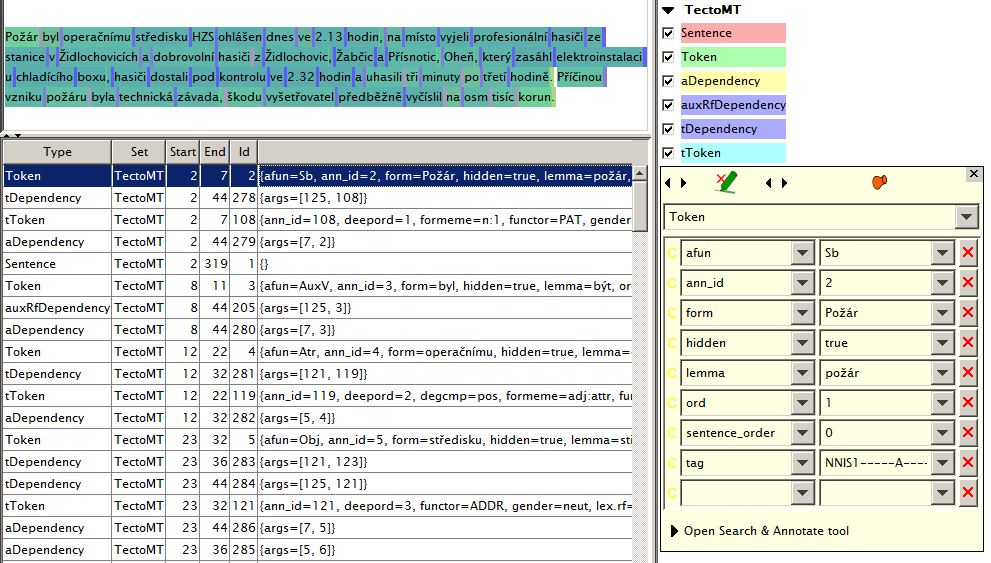
\includegraphics[width=0.7\hsize]{PDT_GATE}}
	\caption{PDT annotations in GATE (screenshot).}
	\label{fig:PDT_GATE}
\end{figure}


\subsubsection{Netgraph Tree Viewer} \label{sec:learning_GATE_Netgraph}

Figure~\ref{fig:GATE_Netgraph}

\begin{figure}
	\centering
		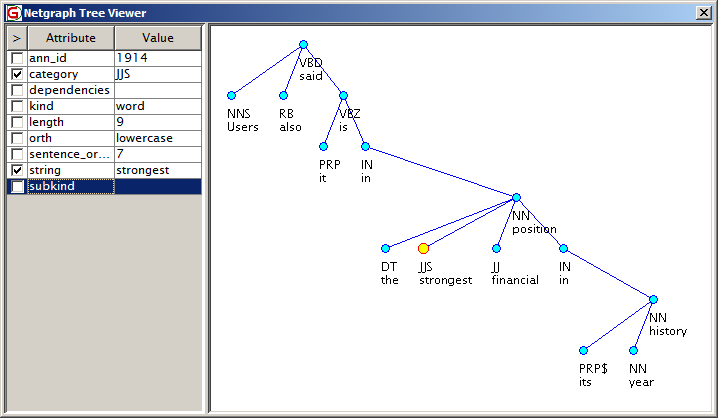
\includegraphics[width=0.7\hsize]{netgraph_stanford}
		\\Sentence: Users also said it is in the strongest financial position in its 24-year history.
	\caption{Netgraph Tree Viewer in GATE (for Stanford Dependencies, screenshot).}
	\label{fig:GATE_Netgraph}
\end{figure}


\subsection{ILP Wrapper (Machine Learning)} \label{sec:learning_ilp_wrapper}
After a human annotator have annotated several documents with desired target annotations, machine learning takes place. 
This consists of two steps: 
\begin{enumerate}
	\item learning of extraction rules from the target annotations and
	\item application of the extraction rules on new documents.
\end{enumerate}
In both steps the linguistic analysis has to be done before and in both steps ILP background knowledge (a logical database of facts) is constructed from linguistic structures of documents that are being processed. We call the process of background knowledge construction as \emph{ILP serialization}; more details are presented below in Section~\ref{sec:learning_ilp_serialization}.

After the ILP serialization is done, the next step depends on the phase which is being performed.

In the learning case, positive and negative examples are constructed from target annotations and the machine learning ILP inductive procedure is executed to obtain extraction rules.

In the application case a Prolog system is used to check if the extraction rules entail any of target annotation candidates.


%Learning / application
%\\1.	serialization -> learning in ILP
%\\2.	serialization -> application in ILP


The learning examples and annotation candidates are usually constructed from all document tokens (and we did so in the present solution), but it can be optionally changed to any other textual unit, for example only numerals or tectogrammatical nodes (words with lexical meaning) can be selected. This can be done easily with the help of \emph{Machine Learning PR} (LM PR) from GATE\footnote{\emph{Machine Learning PR} is an old GATE interface for ML and it is almost obsolete but in contrast to the new \emph{Batch Learning PR} the LM PR is easy to extend for a new ML engine.}.

ML PR provides an interface for exchange of features (including target class) between annotated texts and propositional learners in both directions -- during learning as well as during application. We have used ML PR and developed our \emph{ILP Wrapper} for it. The implementation was a little complicated because complex linguistic structures cannot be easily passed as propositional features, so in our solution we use the ML PR interface only for exchange of the class attribute and annotation id and we access the linguistic structures directly in a document.



\subsection{ILP Serialization} \label{sec:learning_ilp_serialization}

In this section details about conversion of linguistic trees to ILP background knowledge (a Prolog logical database of facts) will be presented. Although the construction is quite strait forward it is worth describing because it makes it easier to understand the extraction rules found by the ILP learning procedure. 

As mentioned in Section~\ref{sec:learning_pdt_in_gate}: three main constructs are used to capture an arbitrary configuration of a dependency linguistic tree: nodes, edges and node attributes. During the process of ILP Serialization these constructs are rendered to Prolog in following way. 

A unique identifier (node ID) is generated for every tree node. The identifier is based on document name and GATE annotation ID.\footnote{Note that node IDs based on sentence order and node deep order are used outside of GATE, see PML$\rightarrow$RDF transformation in Section~\ref{sec:onto_pml_to_rdf}.} These node IDs correspond to simple Prolog atoms and they represent tree nodes in the Prolog fact database. A node type (used by the ILP learning algorithm) is assigned to a node ID by predicates \texttt{Token(NodeID)} for analytical tree nodes and \texttt{tToken(NodeID)} for tectogrammatical tree nodes.

Tree nodes are connected by edges using several binary predicates with a common form:

\texttt{dependency\_type\_name(ParentNodeID, ChildNodeID)}

\noindent Note that the parent (governor) node always occupies the first argument and the child (dependant) node the second one. Predicate name \emph{tDependency} is used for tectogrammatical dependencies and \emph{aDependency} for analytical ones. There are also special kinds of dependencies that connect tectogrammatical and analytical nodes: \emph{lex.rf} (main lexical reference) and \emph{aux.rf} (auxiliary reference), in these cases tectogrammatical node occupies the first argument and analytical the second.

Node attributes are assigned to node IDs by binary predicates of the form:

\texttt{attribute\_name(NodeID, AttributeValue)}

\noindent There are about thirty such predicates like \emph{t\_lemma} (tectogrammatical lemma), \emph{functor} (tectogrammatical functor), \emph{sempos} (semantic part of speech), \emph{negation}, \emph{gender}, etc. but only some of them can be found in example extraction rules and we also excluded some of the attributes from serialization examples for space and simplicity reasons.

Example of a serialized tectogrammatical tree is in Figure~\ref{fig:ilp_serialization} it is the same tree as in Figure~\ref{fig:intro_damage_tree}.

\subsubsection{Attachment of Overlapping GATE Annotations}
During the development of the method, it turned out that it would be very useful to attach additional information, represented by overlapping GATE annotations, to tree nodes. This allows combination of information provided by linguistic trees with information provided by other GATE tools like gazetteers, etc. 

Technically, this is realized using binary predicates with a common form:

\texttt{overlap\_OverlappingType\_OverlappedType(}
\\ \phantom{a} \hfill{} \phantom{b} \texttt{OverlappingAnnotationID, OverlappedNodeID)}

\noindent An overlap with named entities discovers by gazetteers is the most common form of it. For tectogrammatical nodes, it has the form of \texttt{overlap\_Lookup\_tToken(id1,id2)}. An example can be found in Figure~\ref{fig:learning_eval_rules} on line 34. 


%%%%%%%%%%%%%%%%%%%%%%%%%%%%%%%%%%%%%%%%%%%%%%%%%%%%%%%%%%%%%%%%%%%%%%%%%%%%%%%%%%%%%
\begin{figure}
\begin{minted}[linenos, fontsize=\footnotesize,
               frame=lines]{prolog}
tToken(  id_jihomoravsky47443_243).
t_lemma( id_jihomoravsky47443_243, 'být'). %to be
functor( id_jihomoravsky47443_243, 'PRED').
sempos(  id_jihomoravsky47443_243, 'v').
tDependency( id_jihomoravsky47443_243, id_jihomoravsky47443_238).
tToken(  id_jihomoravsky47443_238).
t_lemma( id_jihomoravsky47443_238, ','). %comma
functor( id_jihomoravsky47443_238, 'APPS').
sempos(  id_jihomoravsky47443_238, 'n.denot').
gender(  id_jihomoravsky47443_238, 'nr').
tDependency( id_jihomoravsky47443_238, id_jihomoravsky47443_237).
tToken(  id_jihomoravsky47443_237).
t_lemma( id_jihomoravsky47443_237, 'vyčíslit'). %to quantify
functor( id_jihomoravsky47443_237, 'PAT').
sempos(  id_jihomoravsky47443_237, 'v').
tDependency( id_jihomoravsky47443_237, id_jihomoravsky47443_245).
tToken(  id_jihomoravsky47443_245).
t_lemma( id_jihomoravsky47443_245, 'předběžně'). %preliminarily
functor( id_jihomoravsky47443_245, 'MANN').
sempos(  id_jihomoravsky47443_245, 'adv.denot.grad.nneg').
tDependency( id_jihomoravsky47443_237, id_jihomoravsky47443_244).
tToken(  id_jihomoravsky47443_244).
t_lemma( id_jihomoravsky47443_244, 'vyšetřovatel'). %investigator
functor( id_jihomoravsky47443_244, 'ACT').
sempos(  id_jihomoravsky47443_244, 'n.denot').
gender(  id_jihomoravsky47443_244, 'anim').
tDependency( id_jihomoravsky47443_237, id_jihomoravsky47443_240).
tToken(  id_jihomoravsky47443_240).
t_lemma( id_jihomoravsky47443_240, 'osm'). %eight
functor( id_jihomoravsky47443_240, 'PAT').
sempos(  id_jihomoravsky47443_240, 'n.quant.def').
gender(  id_jihomoravsky47443_240, 'nr').
tDependency( id_jihomoravsky47443_240, id_jihomoravsky47443_242).
tToken(  id_jihomoravsky47443_242).
t_lemma( id_jihomoravsky47443_242, 'tisíc'). %thousand
functor( id_jihomoravsky47443_242, 'RSTR').
sempos(  id_jihomoravsky47443_242, 'n.quant.def').
gender(  id_jihomoravsky47443_242, 'inan').
tDependency( id_jihomoravsky47443_242, id_jihomoravsky47443_247).
tToken(  id_jihomoravsky47443_247).
t_lemma( id_jihomoravsky47443_247, 'koruna'). %crown
functor( id_jihomoravsky47443_247, 'MAT').
sempos(  id_jihomoravsky47443_247, 'n.denot').
gender(  id_jihomoravsky47443_247, 'fem').
tDependency( id_jihomoravsky47443_237, id_jihomoravsky47443_246).
tToken(  id_jihomoravsky47443_246).
t_lemma( id_jihomoravsky47443_246, 'škoda'). %damage
functor( id_jihomoravsky47443_246, 'PAT').
sempos(  id_jihomoravsky47443_246, 'n.denot').
gender(  id_jihomoravsky47443_246,'fem').
\end{minted}
\caption{ILP serialization example based on the tree from Figure~\ref{fig:intro_damage_tree}.}
\label{fig:ilp_serialization}
\end{figure}
%%%%%%%%%%%%%%%%%%%%%%%%%%%%%%%%%%%%%%%%%%%%%%%%%%%%%%%%%%%%%%%%%%%%%%%%%%%%%%%%%%%%%








\clearpage


%%%%%%%%%%%%%%%%%%%%%%%%%%%%%%%%%%%%%%%%%%%%%%%%%%%%%%%%%%%%%%%%%%%%%%%%%%%%%%%%%%%%%
%%%%%%%%%%%%%%%%%%%%%%%%%%%%%%%%%%%%%%%%%%%%%%%%%%%%%%%%%%%%%%%%%%%%%%%%%%%%%%%%%%%%%
%%%%%%%%%%%%%%%%%%%%%%%%%%%%%%%%%%%%%%%%%%%%%%%%%%%%%%%%%%%%%%%%%%%%%%%%%%%%%%%%%%%%%
\section{Shareable Extraction Ontologies} \label{sec:onto_implement}
\graphicspath{{../img/ch70/}}


In this section we will present details about the implementation of our case study with shareable extraction ontologies.  We have used our IE engine based on deep linguistic parsing and Inductive Logic Programming, which was described in Section~\ref{sec:learning_methods}. It is a complex system implemented with a great help of the GATE system and it also uses many other third party tools including several linguistic tools and a Prolog system. Installation and making the system operate is not simple. This case study should demonstrate that the extraction rules produced by the system are not dependent on the system in the sense of shareable extraction ontologies.




\subsection{Linguistic Analysis}



The IE engine needs a linguistic preprocessing (deep linguistic parsing) of documents on its input. Deep linguistic parsing brings a very complex structure to the text and the structure serves as a footing for the construction and application of extraction rules. We usually use TectoMT system to do the linguistic preprocessing, see Section~\ref{sec:third_tectomt} for details. The output linguistic annotations of the TectoMT system are stored (along with the text of the source document) in XML files in so called Prague Markup Language (PML). PML is a very complex language (or XML schema) that is able to express many linguistic elements and features present in text. For the IE engine a tree dependency structure of words in sentences is the most useful one because the edges of the structure guide the extraction rules. Such (tectogrammatical) tree structure was already presented in this thesis, e.g. in Figure~\ref{fig:intro_damage_tree}.


\subsection{Data Transformation (PML to RDF)} \label{sec:onto_pml_to_rdf}

In this case study, PML files made by TectoMT from source documents are transformed to RDF document ontologies by quite simple GRDDL/XSLT transformation\footnote{The transformation is available on-line at \url{http://czsem.berlios.de/ontologies/tmt2rdf.xsl}}. Such document ontology contains the whole variety of PML in RDF format. An example of such document ontology can be seen in Figure~\ref{fig:rdf_serialization}. It shows RDF serialization of the tree presented in Figure~\ref{fig:intro_damage_tree} and transformed to ILP background knowledge in Figure~\ref{fig:ilp_serialization}. Transcript of Czech words is provided in comments.

Figure~\ref{fig:annotated_DO} shows an example of annotated document ontology, which was created by the application of extraction rules on the document ontology from Figure~\ref{fig:rdf_serialization}. Lines 13-15 and 23-25 are added by reasoner; lines 13-15 and 23 are not very interesting, they show some technical constructions based on the schema mapping, but lines 24 and 25 represent the result of extraction rules, these lines mark the corresponding tree node as ``\emph{mention root} of the \emph{damage} task''. The same annotated document ontology is shown on Figure~\ref{fig:PDT_PROTEGE} as a screenshot of the Protégé ontology editor\footnote{\url{http://protege.stanford.edu/}}.



%%%%%%%%%%%%%%%%%%%%%%%%%%%%%%%%%%%%%%%%%%%%%%%%%%%%%%%%%%%%%%%%%%%%%%%%%%%%%%%%%%%%%
\begin{figure}
\begin{minted}[linenos, fontsize=\footnotesize,
               frame=lines, tabsize=2]{turtle}
@prefix node: <http://czsem.berlios.de/ontolog.../jihomoravsky47443.owl#node/> .
@prefix pml: <http://ufal.mff.cuni.cz/pdt/pml/> .

node:SCzechT-s4-n1 rdf:type pml:Node, owl:Thing;
			pml:t_lemma "být" ; #to be
			pml:sempos "v" ; pml:verbmod "ind" ; 
			pml:lex.rf node:SCzechA-s4-w4 ; pml:hasParent node:SCzechT-s4-root .
node:SCzechT-s4-n10 rdf:type pml:Node, owl:Thing;
			pml:t_lemma "vyšetřovatel" ; #investigator
			pml:negation "neg0" ; pml:sempos "n.denot" ;
			pml:gender "anim" ; pml:number "sg" ;
			pml:formeme "n:1" ; pml:functor "ACT" ;
			pml:lex.rf node:SCzechA-s4-w9 ; pml:hasParent node:SCzechT-s4-n8 .
node:SCzechT-s4-n11 rdf:type pml:Node, owl:Thing;
			pml:degcmp "pos" ; pml:t_lemma "předběžně" ; #preliminarily
			pml:formeme "adv:" ; pml:sempos "adv.denot.grad.nneg" ;
			pml:functor "MANN" ; pml:negation "neg0" ;
			pml:lex.rf node:SCzechA-s4-w10 ; pml:hasParent node:SCzechT-s4-n8 .
node:SCzechT-s4-n12 rdf:type pml:Node, owl:Thing;
			pml:t_lemma "osm" ; #eight
			pml:number "pl" ; pml:numertype "basic" ;
			pml:sempos "n.quant.def" ; pml:formeme "n:???" ;
			pml:functor "PAT" ; pml:gender "nr" ;
			pml:lex.rf node:SCzechA-s4-w13 ; pml:hasParent node:SCzechT-s4-n8 .
node:SCzechT-s4-n13 rdf:type pml:Node, owl:Thing;
			pml:t_lemma "tisíc" ; #thousand
			pml:number "sg" ; pml:functor "RSTR" ;
			pml:gender "inan" ; pml:sempos "n.quant.def" ;
			pml:numertype "basic" ; pml:formeme "n:???" ;
			pml:lex.rf node:SCzechA-s4-w14 ; pml:hasParent node:SCzechT-s4-n12 .
node:SCzechT-s4-n14 rdf:type pml:Node, owl:Thing;
			pml:t_lemma "koruna" ; #crown
			pml:gender "fem" ; pml:sempos "n.denot" ;
			pml:number "pl" ; pml:formeme "n:2" ;
			pml:functor "MAT" ; pml:negation "neg0" ;
			pml:lex.rf node:SCzechA-s4-w15 ; pml:hasParent node:SCzechT-s4-n13 .
node:SCzechT-s4-n7 rdf:type pml:Node, owl:Thing;
			pml:t_lemma "," ; #comma
			pml:gender "nr" ; pml:negation "neg0" ;
			pml:sempos "n.denot" ; pml:functor "APPS" ;
			pml:formeme "n:???" ; pml:number "nr" ;
			pml:lex.rf node:SCzechA-s4-w7 ; pml:hasParent node:SCzechT-s4-n1 .
node:SCzechT-s4-n8 rdf:type pml:Node, owl:Thing;
			pml:t_lemma "vyčíslit" ; #quantify
			pml:is_member "1" ; pml:deontmod "decl" ; pml:formeme "v:fin" ;
			pml:tense "ant" ; pml:verbmod "ind" ; pml:aspect "cpl" ;
			pml:is_clause_head "1" ; pml:functor "PAR" ;
			pml:dispmod "disp0" ; pml:sempos "v" ; pml:negation "neg0" ;
			pml:lex.rf node:SCzechA-s4-w11 ; pml:hasParent node:SCzechT-s4-n7 .
node:SCzechT-s4-n9 rdf:type pml:Node, owl:Thing;
			pml:t_lemma "škoda" ; #damage
			pml:sempos "n.denot" ; pml:functor "PAT" ; pml:gender "fem" ;
			pml:formeme "n:4" ; pml:number "sg" ; pml:negation "neg0" ;
			pml:lex.rf node:SCzechA-s4-w8 ; pml:hasParent node:SCzechT-s4-n8 .
\end{minted}
\caption{Document ontology (RDF serialization of linguistic trees), based on Figure~\ref{fig:intro_damage_tree}}.
\label{fig:rdf_serialization}
\end{figure}
%%%%%%%%%%%%%%%%%%%%%%%%%%%%%%%%%%%%%%%%%%%%%%%%%%%%%%%%%%%%%%%%%%%%%%%%%%%%%%%%%%%%%




%%%%%%%%%%%%%%%%%%%%%%%%%%%%%%%%%%%%%%%%%%%%%%%%%%%%%%%%%%%%%%%%%%%%%%%%%%%%%%%%%%%%%
\begin{figure}
\begin{minted}[linenos, fontsize=\footnotesize,
               frame=lines, tabsize=2]{turtle}
@prefix node: <http://czsem.berlios.de/ontologies/.../jihomoravsky47443.owl#node/> .
@prefix pml: <http://ufal.mff.cuni.cz/pdt/pml/> .
# Mapping Ontology
@prefix PML2GATE: <http://czsem.berlios.de/ontologies/PML2GATE_ontology_utils.owl#> .

node:SCzechT-s4-n12 rdf:type pml:Node, owl:Thing;
			 pml:t_lemma "osm" ; #eight
			 pml:number "pl" ; pml:numertype "basic" ;
			 pml:sempos "n.quant.def" ; pml:formeme "n:???" ;
			 pml:functor "PAT" ; pml:gender "nr" ;
			 pml:lex.rf node:SCzechA-s4-w13 ; pml:hasParent node:SCzechT-s4-n8 ;
################### Added by Reasoner ############################################
			 rdf:type PML2GATE:TNode ; #Tectogrammatical node
			 PML2GATE:hasChild node:SCzechT-s4-n13 ;
			 pml:tDependency node:SCzechT-s4-n13 .
##################################################################################
node:SCzechA-s4-w13 rdf:type pml:Node, owl:Thing;
			 pml:is_auxiliary "0" ; pml:edge_to_collapse "1" ;
			 pml:ord "13" ; pml:tag "Cn-S4----------" ;
			 pml:afun "Obj" ; pml:form "osm" ; pml:lemma "osm\1408" ;
			 pml:m.rf node:SCzechM-s4-w13 ; pml:hasParent node:SCzechA-s4-w12 ;
################### Added by Reasoner ############################################
			 PML2GATE:hasChild node:SCzechA-s4-w14 ;
			 pml:mention_root "damage" ;
			 rdf:type PML2GATE:MentionRoot .
##################################################################################
\end{minted}
\caption{Annotated document ontology example}
\label{fig:annotated_DO}
\end{figure}
%%%%%%%%%%%%%%%%%%%%%%%%%%%%%%%%%%%%%%%%%%%%%%%%%%%%%%%%%%%%%%%%%%%%%%%%%%%%%%%%%%%%%

\begin{figure}
\centerline{\framebox{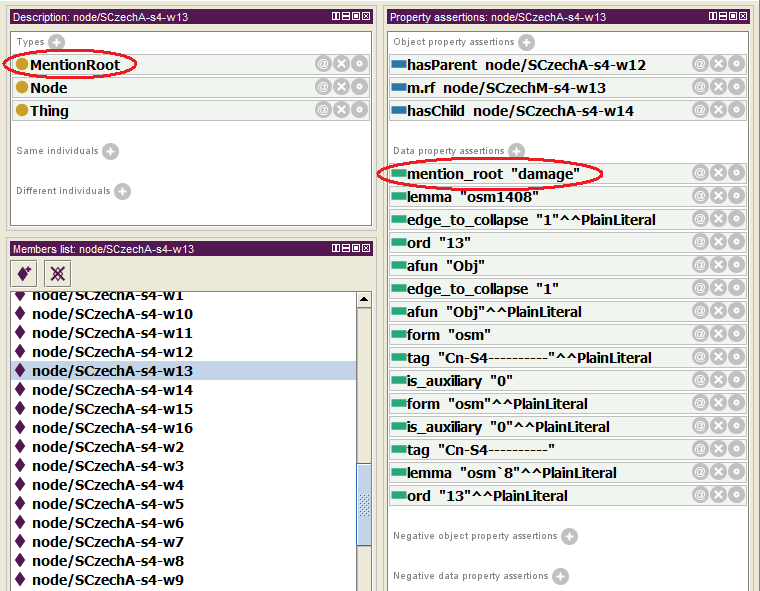
\includegraphics[width=0.7\hsize]{PDT_PROTEGE.png}}}
\caption{Annotated document ontology in Protégé ontology editor}
\label{fig:PDT_PROTEGE}
\end{figure}






\clearpage

\subsection{Rule Transformations}


Extraction rules produced by the IE engine are natively kept in a Prolog format; examples can be seen in Figure~\ref{fig:rules_prolog}. The engine is capable to export them to the OWL/XML\footnote{\url{http://www.w3.org/TR/owl-xmlsyntax/}} syntax for rules in OWL 2 \citep{GHPP09a} (see in Figure~\ref{fig:rules_xml}). Such rules can be parsed by OWL API\footnote{\url{http://owlapi.sourceforge.net/}} 3.1 
and exported to RDF/SWRL, which is very widely supported and hopefully becoming a W3C recommendation.
Figure~\ref{fig:rules_protege} shows the example rules in Prot\'{e}g\'{e} 4 -- Rules View's format. The last rule example can be seen in Figure~\ref{fig:rules_jena}, it shows a rule in the Jena rules format\footnote{\url{http://jena.sourceforge.net/inference/#RULEsyntax}}. Conversion to Jena rules was necessary because it is the only format that Jena can parse, see details about our use of Jena in Section~\ref{sec:onto_experiment}. The Jena rules were obtained using following transformation process:
\begin{enumerate}
	\item OWL/XML $\rightarrow$ RDF/SWRL conversion using OWL API and 
	\item RDF/SWRL $\rightarrow$ Jena rules conversion using SweetRules\footnote{\url{http://sweetrules.semwebcentral.org/}}.
\end{enumerate}


The presented rules belong to the group of so called DL-Safe rules \citep{Motik:DL-Safe-rules} so the decidability of OWL reasoning is kept.




\begin{figure}
\begin{minted}[linenos,  fontsize=\footnotesize,
               frame=lines, tabsize=2]{prolog}
%[Rule 1] [Pos cover = 14 Neg cover = 0]
mention_root(damage,A) :-
   'lex.rf'(B,A), sempos(B,'n.quant.def'), tDependency(C,B), tDependency(C,D), 
   t_lemma(D,'vyšetřovatel'). %investigator

%[Rule 2] [Pos cover = 13 Neg cover = 0]
mention_root(damage,A) :-
   'lex.rf'(B,A), functor(B,'TOWH'), tDependency(C,B), tDependency(C,D), 
   t_lemma(D,'škoda'). %damage
\end{minted}
	\caption{Examples of extraction rules in the native Prolog format.}
	\label{fig:rules_prolog}
\end{figure}


\begin{figure}
\begin{minted}[linenos,  fontsize=\footnotesize,
               frame=lines, tabsize=2]{xml}
<?xml version="1.0" encoding="UTF-8"?>
<!DOCTYPE Ontology [
	<!ENTITY pml "http://ufal.mff.cuni.cz/pdt/pml/" >
]>
<Ontology xmlns="http://www.w3.org/2002/07/owl#"
	ontologyIRI="http://czsem.berlios.de/ontologies/...rules.owl">
	<DLSafeRule>
		<Body>
			<ObjectPropertyAtom> <ObjectProperty IRI="&pml;lex.rf"/>
				<Variable IRI="urn:swrl#b"/> <Variable IRI="urn:swrl#a"/>
			</ObjectPropertyAtom>
			<DataPropertyAtom> <DataProperty IRI="&pml;sempos"/>
				<Variable IRI="urn:swrl#b"/> <Literal>n.quant.def</Literal>
			</DataPropertyAtom>
			<ObjectPropertyAtom> <ObjectProperty IRI="&pml;tDependency"/>
				<Variable IRI="urn:swrl#c"/> <Variable IRI="urn:swrl#b"/>
			</ObjectPropertyAtom>
			<ObjectPropertyAtom> <ObjectProperty IRI="&pml;tDependency"/>
				<Variable IRI="urn:swrl#c"/> <Variable IRI="urn:swrl#d"/>
			</ObjectPropertyAtom>
			<DataPropertyAtom> <DataProperty IRI="&pml;t_lemma"/>
				<Variable IRI="urn:swrl#d"/> <Literal>vyšetřovatel</Literal>
			</DataPropertyAtom>
		</Body>
		<Head>
			<DataPropertyAtom> <DataProperty IRI="&pml;mention_root" />
				<Literal>damage</Literal> <Variable IRI="urn:swrl#a" />
			</DataPropertyAtom>
		</Head>
	</DLSafeRule>
</Ontology>
\end{minted}
\caption{Rule 1 in the OWL/XML syntax for Rules in OWL 2 \citep{GHPP09a}.}
\label{fig:rules_xml}
\end{figure}


\begin{figure}
\begin{minted}[linenos,  fontsize=\footnotesize,
               frame=lines, tabsize=2]{jena}
#[Rule 1]
lex.rf(?b, ?a), sempos(?b, "n.quant.def"), tDependency(?c, ?b),
tDependency(?c, ?d), t_lemma(?d, "vyšetřovatel") #investigator
		-> mention_root(?a, "damage")

#[Rule 2]
lex.rf(?b, ?a), functor(?b, "TOWH"), tDependency(?c, ?b),
tDependency(?c, ?d), t_lemma(?d, "škoda") #damage
		-> mention_root(?a, "damage")
\end{minted}
	\caption{Examples of extraction rules in Prot\'{e}g\'{e} 4 -- Rules View's format.}
	\label{fig:rules_protege}
\end{figure}



\begin{figure}
\begin{minted}[linenos,  fontsize=\footnotesize,
               frame=lines, tabsize=2]{jena}
@prefix pml: <http://ufal.mff.cuni.cz/pdt/pml/>.
[rule-75:  
        ( ?b pml:lex.rf ?a )
        ( ?b pml:sempos 'n.quant.def' )
        ( ?c pml:tDependency ?b )
        ( ?c pml:tDependency ?d )
        ( ?d pml:t_lemma 'vyšetřovatel' )
     -> 
        ( ?a pml:mention_root 'damage' )
]
\end{minted}
\caption{Rule 1 in the Jena rules syntax.}
\label{fig:rules_jena}
\end{figure}


\clearpage










\section{Fuzzy ILP Classification}

In the experimental system we use two inductive logic approaches: crisp and fuzzy (as described above). Technically, the difference between the approaches consists in a different setting of the underlying \emph{ILP task}. Both can be done with a classical ILP tool (Aleph (see Section~\ref{sec:third_ILP_tool}) was used in the final implementation).

We have compared results of the crisp and fuzzy approaches with other classification methods and, in our experiment, the fuzzy approach produced better results than many other methods, including the crisp one. See Section~\ref{sec:fuzzy_results} for details.



\begin{figure}
\begin{minipage}[b]{0.5\hsize}
\begin{minted}[mathescape,fontsize=\footnotesize,
               frame=single]{prolog}
% Crisp learning examples $E_t$

serious_2(id_47443). %positive

serious_0(id_47443). %negative
serious_1(id_47443). %negative
serious_3(id_47443). %negative							

%%%%%%%%%%%%%%%%%%%%%%%%%%%%%%%%%%%%%
% Monotonized learning examples $E_{{\ge}t}$

serious_atl_0(id_47443). %positive
serious_atl_1(id_47443). %positive
serious_atl_2(id_47443). %positive

serious_atl_3(id_47443). %negative					
\end{minted}						
	\caption{Learning examples.}
	\label{fig:examples}
\end{minipage}
\hspace{0.5cm}
\begin{minipage}[b]{0.5\hsize}
\begin{minted}[fontsize=\footnotesize,
               frame=single]{prolog}
size(id_47443, 427).
type(id_47443, fire).
damage(id_47443, 8000).
dur_minutes(id_47443, 50).
fatalities(id_47443, 0).
injuries(id_47443, 0).
cars(id_47443, 0).
amateur_units(id_47443, 3).
profesional_units(id_47443, 1).
pipes(id_47443, unknown).
lather(id_47443, 0).
aqualung(id_47443, 0).
fan(id_47443, 0).
\end{minted}						
	\caption{$B^{crisp}_{T}$ -- crisp attributes.}
	\label{fig:crisp_attributes}
\end{minipage}
\end{figure}






To use ILP for a classification task we have to translate the input data to the Prolog-like logic representation, as it was already described in previous sections. Here we will describe implementation details of constructing crisp and fuzzy knowledge bases and example sets.

In construction of a crisp example set $E_t$, the target predicate is denoted as \texttt{serious\_t}. The letter \texttt{t} stands for the actual seriousness degree. We use multiple unary predicates \texttt{serious\_0}, \texttt{serious\_1}, etc., instead of one binary predicate \texttt{serious(ID,Degree)}. These two cases are equivalent and we have decided to use the unary option because a visual distinction between the multiple ILP tasks is then clearer.

In construction of a fuzzy (or monotonized) example set $E_{\ge t}$, the target predicate is denoted as \texttt{serious\_atl\_t}, see examples in Figure~\ref{fig:examples}.



In construction of a crisp background knowledge $B^{crisp}_{T}$, we use a~simple translation of the attribute names to the names of predicates and fill them with actual values. It is illustrated in Figure~\ref{fig:crisp_attributes}). 



In construction of a monotonized background knowledge $B^{monot}_T$ we reuse the crisp background knowledge and add monotonization rules. An~example for predicate \texttt{damage} is shown in Figure~\ref{fig:attribute_monotonization}.
%on predicates \texttt{damage} and \texttt{damage\_atl}.
The first rule deals with \texttt{unknown} values (Section~\ref{sec:data_features} deals with unknown values in the dataset) and the second does the monotonization. 

Negations used in Figure~\ref{fig:attribute_monotonization} and Figure~\ref{fig:conversion} are the standard Prolog \emph{negations as failure}.



\begin{figure}	
\begin{minted}[fontsize=\footnotesize,
               frame=lines, tabsize=2]{prolog}
damage_atl(ID,N) :- damage(ID,N), not(integer(N)). %unknown values

damage_atl(ID,N) :- damage(ID,N2), integer(N2), %numeric values
                    damage(N), integer(N), N2>=N.
\end{minted}						
	\caption{Monotonization of attributes (damage\_atl $\leftarrow$ damage).}
	\label{fig:attribute_monotonization}
\end{figure}


\begin{figure}
\begin{minted}[linenos,  fontsize=\footnotesize,
               frame=lines]{prolog}
serious_0(A) :- fatalities(A,0), injuries(A,0), cars(A,1), amateur_units(A,0), lather(A,0).
serious_0(A) :- fatalities(A,0), cars(A,0), amateur_units(A,0), professional_units(A,1).
serious_1(A) :- amateur_units(A,1).
serious_1(A) :- damage(A,300000).
serious_1(A) :- type(A,fire), amateur_units(A,0), pipes(A,2).
serious_1(A) :- type(A,car_accident),dur_minutes(A,unknown),fatalities(A,0),injuries(A,1).
serious_2(A) :- lather(A,unknown).
serious_2(A) :- cars(A,0), lather(A,0), aqualung(A,1), fan(A,0).
serious_2(A) :- amateur_units(A,2).
serious_3(A) :- fatalities(A,2).
serious_3(A) :- type(A,fire), dur_minutes(A,unknown), cars(A,0), fan(A,0).
serious_3(A) :- injuries(A,2), cars(A,2).
serious_3(A) :- fatalities(A,1).

serious_atl_0(A).
serious_atl_1(A) :- injuries_atl(A,1).
serious_atl_1(A) :- dur_minutes_atl(A,21), pipes_atl(A,1), aqualung_atl(A,0).
serious_atl_1(A) :- damage_atl(A,8000), amateur_units_atl(A,3).
serious_atl_1(A) :- dur_minutes_atl(A,197).
serious_atl_1(A) :- dur_minutes_atl(A,unknown).
serious_atl_2(A) :- dur_minutes_atl(A,50), pipes_atl(A,3).
serious_atl_2(A) :- size_atl(A,1364), injuries_atl(A,1).
serious_atl_2(A) :- fatalities_atl(A,1).
serious_atl_2(A) :- size_atl(A,1106), professional_units_atl(A,3).
serious_atl_3(A) :- fatalities_atl(A,1).
serious_atl_3(A) :- damage_atl(A,1500000).
\end{minted}
\caption{Crisp and monotonized hypotheses.}
\label{fig:rules}
\end{figure}


\begin{figure}	
\begin{minted}[fontsize=\footnotesize,
               frame=lines, tabsize=2]{prolog}
serious_0(ID) :- serious_atl_0(ID),
                 not(serious_atl_1(ID)), not(serious_atl_2(ID)), not(serious_atl_3(ID)).
serious_1(ID) :- serious_atl_1(ID),
                 not(serious_atl_2(ID)), not(serious_atl_3(ID)).
serious_2(ID) :- serious_atl_2(ID),
                 not(serious_atl_3(ID)).
serious_3(ID) :- serious_atl_3(ID).
\end{minted}						
\caption{Conversion rules for monotonized hypotheses (serious\_t $\leftarrow$ serious\_atl\_t).}
\label{fig:conversion}
\end{figure}



Once we have learning examples and background knowledge, we can run the ILP inductive procedure and obtain learned rules (a learned hypothesis). According to the kind of the ILP task (crisp or monotonized), we obtain the corresponding kind (crisp or monotonized) of rules (see e.g. in Figure~\ref{fig:rules}). But these rules cannot be used directly to solve the classification task. There are common cases when more than one rule is applicable to a single instance. So we have to select which one to use. For the monotonized hypothesis we select the one with the biggest return value; it is illustrated in Figure~\ref{fig:conversion}. Such clear criterion does not exist for the crisp hypothesis, so we simply use the first applicable rule.


In the crisp case there are often many instances which cannot be classified because there is no applicable rule. In our experiment there was about a 51\%
of unclassified instances (see in the next section). It could be caused by the lack of training data, but the monotonized approach does not suffer from this shortage. We can always select the bottom value.

Another advantage of the monotonized approach is that the set of positive training examples is extended by monotonization. 





%%%%%%%%%%%%%%%%%%%%%%%%%%%%%%%%%%%%%%%%%%%%%%%%%%%%%%%%%%%%%%%%%%%%%%%%%%%%%%%%%%%%%%%%%%%%%%%%%
\subsection{Learned Rules Examples} \label{sec:fuzzy_results}
%%%%%%%%%%%%%%%%%%%%%%%%%%%%%%%%%%%%%%%%%%%%%%%%%%%%%%%%%%%%%%%%%%%%%%%%%%%%%%%%%%%%%%%%%%%%%%%%%

Figure~\ref{fig:rules} summarizes obtained hypotheses learned from our data: 
\begin{itemize}
	\item a crisp hypothesis learned from $E_t$ and $B^{crisp}_{T}$ (lines 1-13) and
	\item a monotonized hypothesis learned from $E_{\ge t}$ and ${B}^{monot}_T$ (lines 15-26).
\end{itemize}


In both cases, learning examples and background knowledge have the origin in the same data (the same accidents). The hypotheses differ in the form of the ILP task (crisp and monotonized). The crisp hypothesis uses only the crisp predicates, and the monotonized hypothesis uses only the monotonized predicates.




